\documentclass[crop]{standalone}

\usepackage{verbatim}

\usepackage{pgfplots}
\usepackage{pgfplotstable}

\usepackage[]{xcolor}

\pgfplotsset{compat=1.8} %v=1.8 required for this plot

\pgfplotstableset{
    create on use/accumyprev/.style = {
        create col/expr = {	\prevrow{0}+
        					\prevrow{1}+
        					\prevrow{2}+
        					\prevrow{3}+
        					\prevrow{4}+
        					\prevrow{5}+
        					\prevrow{6}+
        					\prevrow{7}+
        					\prevrow{8}+
        					\prevrow{9}+
        					\prevrow{10}+
        					\prevrow{11}+
        					\prevrow{12}+
        					\pgfmathaccuma}
    }
}

\begin{document}

\begin{tikzpicture}
\begin{axis}[
 %Plot Type
    ybar stacked,
    bar width=23pt,
%Size
    width=595pt,
    height=350pt,
%Domain
    enlarge x limits=0.04,
    ymin=0, ymax=1,
%???
    %point meta = explicit,
%Ticks and Labels
    xtick = data,
    xticklabel style={rotate=90, align=right, anchor=east},
    xticklabels = { Electrical \\ INPUT,
    				Forward \\ Voltage Loss,
    				Internal \\ Nonradiative Loss,
    				Droop,
    				Unextracted Light,
    				\textcolor{blue}{Blue Light:} \\ Scat.\& Absorption,
    				\textcolor{red}{Red Phosphor:} \\ Nonradiative Loss,
    			    \textcolor{red}{Red Phosphor:} \\ Stokes Loss,
    				\textcolor{red}{Red Phosphor:} \\ Scat.\& Absorption,
    				\textcolor{teal}{Green Phosphor:} \\ Nonradiative Loss,
    				\textcolor{teal}{Green Phosphor:} \\ Stokes Loss,
    				\textcolor{teal}{Green Phosphor:} \\ Scat.\& Absorption,
    				Spectral Loss,
    				Light \\ OUTPUT},
%Axes and Labels
    axis on top,
    ylabel = {Energy [W]},
]
% The first plot sets the "baseline":
% Uses the sum of all previous y values,
% except for the last bar, where it becomes 0
\addplot[
    y filter/.code = {\ifnum\coordindex>12 \def\pgfmathresult{0}\fi},
    draw = none,
    fill = none
] table [col sep=comma, x expr = \coordindex, y = accumyprev] {../data/2016/2016.csv};

\addplot[fill=yellow,draw=black,ybar stacked] table [col sep=comma, x expr = \coordindex, y index = 0, meta index = 0] {../data/2016/2016.csv};
\addplot[fill=lightgray,draw=black,ybar stacked] table [col sep=comma, x expr = \coordindex, y index = 1, meta index = 1] {../data/2016/2016.csv};
\addplot[fill=gray,draw=black,ybar stacked] table [col sep=comma, x expr = \coordindex, y index = 2, meta index = 2] {../data/2016/2016.csv};
\addplot[fill=darkgray,draw=black,ybar stacked] table [col sep=comma, x expr = \coordindex, y index = 3, meta index = 3] {../data/2016/2016.csv};
\addplot[fill=orange,draw=black,ybar stacked] table [col sep=comma, x expr = \coordindex, y index = 4, meta index = 4] {../data/2016/2016.csv};
\addplot[fill=blue,draw=black,ybar stacked] table [col sep=comma, x expr = \coordindex, y index = 5, meta index = 5] {../data/2016/2016.csv};
\addplot[fill=red,draw=black,ybar stacked] table [col sep=comma, x expr = \coordindex, y index = 6, meta index = 6] {../data/2016/2016.csv};
\addplot[fill=red,draw=black,ybar stacked] table [col sep=comma, x expr = \coordindex, y index = 7, meta index = 7] {../data/2016/2016.csv};
\addplot[fill=red,draw=black,ybar stacked] table [col sep=comma, x expr = \coordindex, y index = 8, meta index = 8] {../data/2016/2016.csv};
\addplot[fill=green,draw=black,ybar stacked] table [col sep=comma, x expr = \coordindex, y index = 9, meta index = 9] {../data/2016/2016.csv};
\addplot[fill=green,draw=black,ybar stacked] table [col sep=comma, x expr = \coordindex, y index = 10, meta index = 10] {../data/2016/2016.csv};
\addplot[fill=green,draw=black,ybar stacked] table [col sep=comma, x expr = \coordindex, y index = 11, meta index = 11] {../data/2016/2016.csv};
\addplot[fill=white,draw=black,ybar stacked] table [col sep=comma, x expr = \coordindex, y index = 12, meta index = 12] {../data/2016/2016.csv};
\addplot[fill=yellow,draw=black,ybar stacked] table [col sep=comma, x expr = \coordindex, y index = 13, meta index = 13] {../data/2016/2016.csv};

% The connecting line. Uses a bit of magic to typeset the ranges
  \addplot [
    const plot, black,
    point meta = {
        TeX code symbolic = {
            \pgfkeys{/pgf/fpu/output format=fixed}
            \pgfmathtruncatemacro\upperbound{
                \thisrowno{0}+
                \thisrowno{1}+
                \thisrowno{2}+
                \thisrowno{3}+
                \thisrowno{4}+
                \thisrowno{5}+
                \thisrowno{6}+
                \thisrowno{7}+
                \thisrowno{8}+
                \thisrowno{9}+
                \thisrowno{10}+
                \thisrowno{11}+
                \thisrowno{12}+
                \thisrowno{13}
            }
            \edef\dostuff{
                \noexpand\def\noexpand\pgfplotspointmeta{%
                    \thisrowno{0}--\upperbound%
                }
            }%
            \dostuff
        }
    },
  ] table [col sep=comma, x expr = \coordindex, y expr = 0] {../data/2016/2016.csv};

\end{axis}

\begin{axis}[
%Plot Type
    enlarge x limits=0.04,
%Size
    width=595pt,
    height=350pt,
%Domain
    ymin=0, ymax=1,
%Ticks and Labels
    xticklabels={,,},
    xtick = data,
    major tick length = 0pt,
%Axes and Labels
    visualization depends on={value \thisrow{label} \as \labela},
    nodes near coords={\labela},
]
\addplot [scatter, only marks, no markers] table [col sep=comma, x expr = \coordindex, y=y] {../data/2016/labels1.csv};
\end{axis}

\begin{axis}[
%Plot Type
    enlarge x limits=0.04,
%Size
    width=595pt,
    height=350pt,
%Domain
    ymin=0, ymax=1,
%Ticks and Labels
    xticklabels={,,},
    xtick = data,
    major tick length = 0pt,
%Axes and Labels
    visualization depends on={value \thisrow{label} \as \labela},
    nodes near coords={\labela},
]
\addplot [scatter, only marks, no markers] table [col sep=comma, x expr = \coordindex, y=y] {../data/2016/labels2.csv};
\node [above right] at (rel axis cs:0.58,0.675) {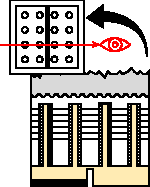
\includegraphics[width=2.5cm]{../data/package/2016_chip.pdf}};
\end{axis}

\begin{axis}[
%Grouping
    at={(1465,185)},
	height=150pt,
	width=150pt,
%Domain
	ymin=0, ymax=1,
	xmin=400, xmax=750,
%Axis Labels
	xlabel style = {align=center},
	ylabel={Intensity [Arb.Units]},
	xlabel={Wavelength [nm]} \\ {YAG:Ce$^{3+}$+PFS},
			]
\addplot [red]
	table [col sep=comma, x=wavelength, y=sensitivity]
	{../data/phosphor/luminosity.csv};
\addplot []
	table [col sep=comma, x=wavelength, y=intensity]
	{../data/phosphor/2015_ge_pfs.csv};
\end{axis}

\end{tikzpicture}

\end{document}
